\documentclass[11pt,oneside,a4paper]{article}
\usepackage{graphicx}
\usepackage{booktabs}
\usepackage{caption}
\usepackage{subcaption}
\usepackage{amsmath}
\usepackage{amsfonts}
\usepackage{amssymb}
\usepackage{lscape}
\usepackage{psfrag}
\usepackage{mathtools}
\usepackage[usenames]{color}
\usepackage{bbm}
\usepackage[update]{epstopdf}
\usepackage[bookmarks,pdfstartview=FitH,a4paper,pdfborder={0 0 0}]{hyperref}
\usepackage{verbatim}
\usepackage{listings}
\usepackage{textcomp}
\usepackage{fancyhdr}
\usepackage{multirow}
\pagestyle{fancy}
\usepackage{tikz}
\usepackage{course}
\usepackage{csvsimple}
\usepackage{float}

\renewcommand{\sectionmark}[1]{\markboth{#1}{#1}}
\renewcommand{\subsectionmark}[1]{\markright{#1}}

\fancyhf{}
\fancyhead[RO]{\nouppercase{\footnotesize\sc\leftmark\ \hrulefill\ \thepage}}
\fancyhead[RE]{\nouppercase{\footnotesize\sc\thepage\ \hrulefill\ }}
\renewcommand{\headrulewidth}{0pt}

\makeatletter
\def\cleardoublepage{\clearpage\if@twoside \ifodd\c@page\else%
	\hbox{}%
	\thispagestyle{empty}%
	\clearpage%
	\if@twocolumn\hbox{}\clearpage\fi\fi\fi}
\makeatother


\renewcommand{\topfraction}{0.9}  % max fraction of floats at top
\renewcommand{\bottomfraction}{0.8} % max fraction of floats at bottom
% Parameters for TEXT pages (not float pages):
\setcounter{topnumber}{2}
\setcounter{bottomnumber}{2}
\setcounter{totalnumber}{4}            % 2 may work better
\setcounter{dbltopnumber}{2}           % for 2-column pages
\renewcommand{\dbltopfraction}{0.9}    % fit big float above 2-col. text
\renewcommand{\textfraction}{0.07}     % allow minimal text w. figs
% Parameters for FLOAT pages (not text pages):
\renewcommand{\floatpagefraction}{0.7}  % require fuller float pages
% N.B.: floatpagefraction MUST be less than topfraction !!
\renewcommand{\dblfloatpagefraction}{0.7} % require fuller float pages

\sloppy

\widowpenalty=10000
\clubpenalty=10000

\edef\today{%\number\day\
	\ifcase\month\or
	January\or February\or March\or April\or May\or June\or July\or
	August\or September\or October\or November\or December\fi\ \number\year}
\title{\vspace*{40.0mm}
	\bf\sf Design of a structured product
	\vspace*{20.0mm} \\
	\vspace*{40.0mm}
	%\vspace{-20mm}\framebox{DRAFT VERSION}\vspace{20mm} \\
	% \Large\bf\sf Design of a structured product \vspace*{20.0mm}}
}
\author{\sf Tim Buchholz}
\date{\sf 21.10.20}

\begin{document}
	
	\begin{figure}
		\parbox[t]{125mm}{
			\vspace*{6mm}
			\scriptsize\sf           FACULTY OF ENGINEERING SCIENCE\\
			\scriptsize\sf\bfseries  Fundamentals of Financial Mathematics \\
			\scriptsize\sf           Home Assignment 2020-2021 \\
			\scriptsize\sf           Tim Buchholz}
		\parbox[t]{40mm}{
			\begin{flushright}
				
\includegraphics[height=15mm]{logo-eps-converted-to.pdf}
		\end{flushright}}
	\end{figure}
	
	\maketitle
	\thispagestyle{empty}
	\raggedbottom
	
	\cleardoublepage
	\pagenumbering{roman}
	\setcounter{tocdepth}{2}
	
	\tableofcontents
	
	\cleardoublepage
	\pagenumbering{arabic}
	
	\section{Introduction, Assumptions and relevant market data}
	In this assignment the design of two structured products for an underlying stock will be discussed. Namely the underlying stock is Advanced Micro Devices, Inc. , which is also known as AMD. AMD is an American multinational semiconductor company, which produces Computer processors and related technologies for business and consumer markets. 
	For many investors AMD is a really interesting company, as it is beside of Intel (Intel Corp. v. Advanced Micro Devices) the biggest producer for computer processors with even growing partial of the market. 
	Additionally the recent release of the new graphics processing units (GPUs) is very promising as these represent serious competition to Nvidia graphics cards, which dominated the market in the last years.
	
	Following structured products will be introduced:
	\begin{itemize}
		\item Product 1: Partially principal protected note
		\item Product 2: Airbag note
	\end{itemize}
	As underlying Finance instruments we will basically consider three different assets:
	\begin{itemize}
		\item the risk-free bank account with an fixed interest rate $r$
		\item the stock $ S $ (in this case AMD)
		\item Call and Put options on the stock S
	\end{itemize}
	As starting date $ t=0 $ Friday the 20st November is choosen.
	The maturity date of the products is Friday 21st January 2022.
	More precisely the structured product, which will be discussed later, are build on the data presented below, accessed at Friday 20st November at 4:45 pm (MEZ), which is one hour and a quarter after the market opening at that day. The stock price at this moment was $ S_0=85.35 \text{ USD} $. The data is shown in the tables at the end of this section. A small extract of the data is moreover shown in a associated screenshot in the appendix. As the tables already contain the full data, the screenshot only shows the stock price and the first few call options.  \\


	To get a fixed interest rate for the whole time period, the daily treasure yield rate of the US treasure bond at the starting date $ t=0 $ is picked, which we denote by $ r = 0.11 \% $.
	In the appendix also an associated table is shown, which is published at \cite{site_treasure}
    an official website of the United States Government.
   
	
	
	The reason of choice is that the base interest rate of the United States, the United States Fed Funds Rate, is given by a target range of $ 0-0.25 \% $. Moreover the Daily Treasury Yield Curve Rates are given for different time periods exactly. Since the time period of our products is around one year and two months the rate for an investment over one year is picked. As the investment is even longer than one year, that is a rather cautious estimate for the interest rate.
	
	
		\begin{table*}[!ht]
		\csvreader[%
		tabular={|c|c|c|c|c|c|c|},
		table head = \hline\textbf{{LastTradeDate}} & \textbf{Strike} & \textbf{LastPrice} & \textbf{Bid} & \textbf{Ask}  & \textbf{Volume} & \textbf{ImpliedVolatility}\\\hline,
		late after line= \\,
		late after last line=\\\hline %
		]{../data/yahoo_pc_stat_210122_table0_20112020_16:45:35}{LastTradeDate=\LastTradeDate,Strike=\Strike,LastPrice=\LastPrice,Bid=\Bid,Ask=\Ask,Volume=\Volume,ImpliedVolatility=\ImpliedVolatility}%
		{\LastTradeDate &\Strike & \LastPrice & \Bid & \Ask & \Volume & \ImpliedVolatility}
		\centering
		\caption{\label{table1}European Call Options AMD (data extracted from \cite{site_yahoofinance} at 20/11/2020 16:45:35)}
	\end{table*}
	\begin{table*}[!ht]
		\csvreader[%
		tabular={|c|c|c|c|c|c|c|c|},
		table head = \hline\textbf{{LastTradeDate}} & \textbf{Strike} & \textbf{LastPrice} & \textbf{Bid} & \textbf{Ask} & \textbf{Volume} & \textbf{ImpliedVolatility}\\\hline,
		late after line= \\,
		late after last line=\\\hline %
		]{../data/yahoo_pc_stat_210122_table1_20112020_16:45:35}{LastTradeDate=\LastTradeDate,Strike=\Strike,LastPrice=\LastPrice,Bid=\Bid,Ask=\Ask,Volume=\Volume,ImpliedVolatility=\ImpliedVolatility}%
		{\LastTradeDate &\Strike & \LastPrice & \Bid & \Ask & \Volume & \ImpliedVolatility}
		\centering
		\caption{\label{table2}European Put Options AMD (data extracted from \cite{site_yahoofinance} at 20/11/2020 16:45:35)}
	\end{table*}
	\newpage
	\section{Product 1: Partially principal protected note (PPPN)}
	\subsection{Descriptive part: What is a PPPN and why is it interesting?}
	A partially principal protected note (PPPN) is an investment option over an underlying stock, in our case AMD. Many people are initially skeptical when it comes to investing in stocks. The reason for this is that the opportunities come with risks. A PPPN is en investment option, where the risk is partially absorbed. For instance imagine investing $850 \text{ USD}$ in a PPPN with fixed maturity date $ T $ over an underlying stock with initial stock price $ S_0 = 85 \text{ USD} $.\\
	 If one would buy the stock directly this would mean buying ten stocks. If at maturity the stock is up to a value of $ 110 \text{ USD} $ one would have a profit of $ 1100 \text{ USD} - 850 \text{ USD} = 250 \text{ USD}  $. But in the case of $ S_T = 60 \text{ USD} $ one would loose the same amount of money.
	 The PPPN is preventing exactly that: One cannot loose more then $ 10 \% $ of the initial investment. But additionally there is profit if the stock rises above a certain strike and if the stock falls below another fixed strike. The following plot explains what exactly is meant for the example situation above ($ S_0 = 85 \text{ USD}$ and an initial investment of $ 850 \text{ USD} $ with strikes $ K_1 = 60\text{ USD} $ and  $ K_2 = 110\text{ USD} $): 
	\begin{figure}[H]
		\centering
		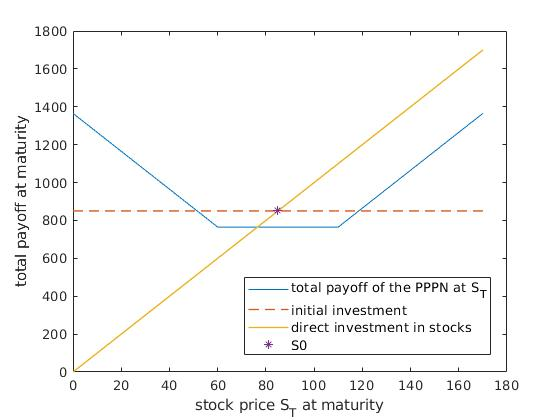
\includegraphics[width=0.8\linewidth]{payoff_PPPN.jpg}
		 \caption{payoff for an PPPN}
	\end{figure} 
	The yellow line represents the direct investment in the stock, where the blue line represents the total payoff of the PPPN. One can see that there is less risk but one has to pay with a smaller profit in the case of a rising stock and a possible loss of up to $ 10 \% $ if the stock stays close to $ S0 $.  Therefore one can get profit even in the case that the stock goes down.
	\newpage
	\subsection{Concrete product}
	The concrete product which can be offered has the following specifications:
	\begin{itemize}
		\item Since the underlying stock is AMD, consider $ S_0 = 85.35 \text{ USD} $.
		\item The investment can be any multiple of $ N = 85.35 \text{ USD} $ which is the stock price $ S_0 $.
		\item The maturity date is $ 21st $ January $ 2022 $ so the duration $ T = 14 $ months.
		\item As lower strike $ K_1 = 40 \text{ USD} $ is picked.
		\item As higher strike $ K_2 = 130 \text{ USD} $ is picked.
	\end{itemize}
	Then the total payoff can be visualized in the same way as in the descriptive part:
	\begin{figure}[H]
		\centering
		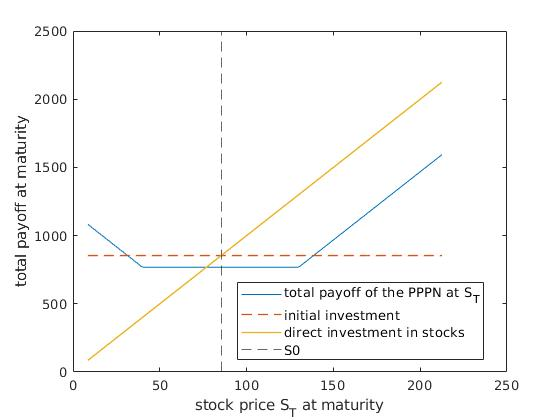
\includegraphics[width=0.8\linewidth]{PPPN_concrete.jpg}
		\caption{payoff for the concrete PPPN offer}
	\end{figure} 
	If the stock goes up $ 100 \% $ till the maturity day one would end up with $ 117.52 \text{ USD}$ for an investment of  $ N = 85.35 \text{ USD} $ . And no matter how the stock moves in the next $ 14 $ months one can never end up with less than $ 76.5 \text{ USD} $.
	\subsection{Technical Part: How does a PPPN work?}
	A PPPN is the combination of three different assets:
	\begin{itemize}
		\item A risk free asset with interest rate $ r $.
		\item Call options on the underlying stock.
		\item Put options on the underlying stock.
	\end{itemize}
	First we have to determine the part of the investment which has to be invested in a risk free way. Therefore we have to discount $ 90 \% $ of the initial investment by the interest rate $ r $ over the time period $ T $. In our case we consider an investment in the US Treasure Bond of 
	\[
		N_{\text{fixed}} = 0.9 N\cdot\exp(-rT) = 0.9  \exp(-0.0011\frac{14}{12}) N = 0.89885 N \ .
	\]
	It remains to invest \[ N_{\text{options}} \leq N-N_{\text{fixed}} = 0.10115N \ . \]
	We are now buying $ \frac{N}{S_0} $ European Put options for the considered maturity date with strike $ K_1 = 40 \text{ USD} $ and the same amount of European Call options for the considered maturity date with strike $ K_2 = 130 \text{ USD} $. To look up the prices of these we have to look up the tables of relevant market data stated above. We can find for the Put option
	\begin{tabular}{|c|c|c|c|c|c|c|}
		\hline\textbf{{LastTradeDate}} & \textbf{Strike} & \textbf{LastPrice} & \textbf{Bid} & \textbf{Ask} & \textbf{Volume} & \textbf{ImpliedVolatility}\\\hline
		2020-11-19 3:08PM EST & 40.0 & 1.42 & 1.35 & 1.5 & 152 & 53.05\%
		\\\hline
	\end{tabular}\\
	and for the Call option
    $\newline$
	\begin{tabular}{|c|c|c|c|c|c|c|}
		\hline\textbf{{LastTradeDate}} & \textbf{Strike} & \textbf{LastPrice} & \textbf{Bid} & \textbf{Ask} & \textbf{Volume} & \textbf{ImpliedVolatility}\\\hline
		2020-11-19 3:57PM EST & 130.0 & 6.95 & 6.6 & 6.95 & 457 & 49.87\%
		\\\hline
	\end{tabular}
	Since we chose $ N $ as a multiple of the initial stock price $ S_0 $ the ratio $ a = \frac{N}{S_0} $ gives us a natural number which is the amount of each Call and Put options we have to buy.
	With the ask prices of the options we get 
	\begin{align*}
	c_{\text{put,ask}} &= 1.5 \text{ USD} \approx 0.017575 S_0 \\
	c_{\text{cal,ask}} &= 6.95 \text{ USD} \approx 0.081429 S_0  \\
	N_{\text{options}} &= \frac{N}{S_0} 0.017575 S_0 + \frac{N}{S_0} 0.081429 S_0 \approx 0.099004 N
	\end{align*}
	The remaining amount  is then a small profit for the bank for selling the option. For  Let us now have a look at the payoff of those three assets at maturity:
	\begin{itemize}
		\item The risk free asset will end up at $ 0.9\cdot N $.
		\item Each of the $ a $ Put options generates a payoff at maturity of $ p_{\text{put}} = (K_1-S_T)^{+} $.
		\item Each of the $ a $ Call options generates a payoff at maturity of $ p_{\text{call}} = (S_T- K_2)^{+} $.
	\end{itemize}
	Thus the total payoff is given by
	\begin{align*}
		p_{\text{total}} &= 0.9\cdot	N + a \cdot p_{\text{put}} + a \cdot p_{\text{call}} \\ &= 0.9N + a\cdot((K_1-S_T)^+ + (S_T- K_2)^+) \\
		&=
		\begin{cases}
				0.9N + \frac{N}{S_0}(K_1 - S_T) \; &\text{if } S_T < K_1 \\
				0.9N  \; &\text{if } K_1 \leq S_T \leq K_2 \\
				0.9N + \frac{N}{S_0}(S_T-K_2) \; &\text{if }S_T > K_2 \\
		\end{cases} \\
	\end{align*}
	and the bank just delivers to the investor the payoff in every case. 
	For an investment of \[N = 10\cdot S_0 = 853.5 \text{ USD} \] this would give the bank a profit of around $ 1.8352 \text{ USD} $ by having nearly no risk.
	
	
	

	\newpage
	\section{Product 2: Airbag note (AN)}
	\subsection{Descriptive part: What is a AN and why is it interesting?}
	\subsection{Technical Part: How does a AN work?}
	\cleardoublepage
	\section{Appendix}
	\subsection{Screenshot of the market data}
	\begin{figure}[H]
		\centering
		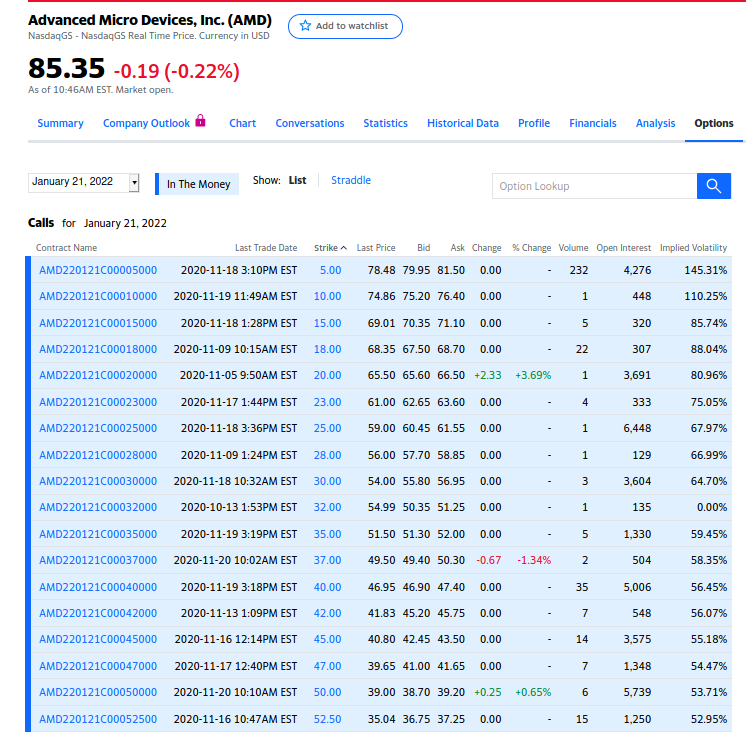
\includegraphics[width=\linewidth]{screenshot.png}
		\caption{\label{treasure}Small extract of the relevant market data from \cite{site_yahoofinance}} 
	\end{figure}
	\subsection{Daily Treasury Yield Curve Rates}
	\begin{figure}[H]
		\centering
		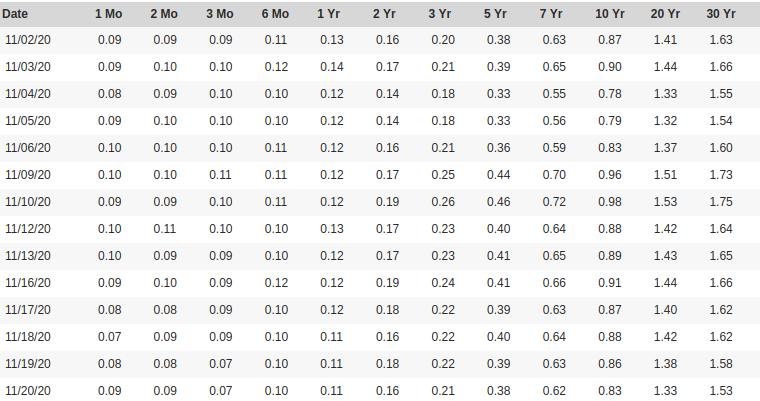
\includegraphics[width=0.8\linewidth]{treasure.png}
		\caption{\label{treasure}Daily Treasury Yield Curve Rates from \cite{site_treasure}} 
	\end{figure}
	\newpage
	\bibliographystyle{abbrv}
	\bibliography{References}
	
	 
\end{document}